\chapter{Spielgerät und Zubehör}
\label{tisch}


%%%%%%%%%%%%%%%%%%%%%%%%%%%%%%%%%%%%%%%%%%%%%%
\section{Der Tisch}
\label{tisch:tisch}

Der Tisch zusammen mit einem Ball ist das Spielgerät beim Tischfußball. 
Das etwa 1,1 m lange und 0,7 m breite Spielfeld ist im Tischkorpus, der auf vier Beinen steht, eingelassen und von Banden umrundet. An den Stirnseiten sind die Tore platziert, die mit einer Torauffangschale oder einem Ballrücklauf ausgestattet sind.  
Die jeweils 11 Spielfiguren sind auf 4 Stangen (für drei Spielbereiche) verteilt:
\begin{itemize}  
\item die Torwartstange, auch Torwart (\gls{abwehr}) 
\item die 2er-Stange, auch die Zwei (\gls{abwehr}) 
\item die 5er-Stange, auch die Fünf (\gls{mittelfeld})
\item die 3er-Stange (\gls{sturm})
\end{itemize}  
Die Stangen können mittels Griffen vor- und zurückgedreht und rein- und rausgeschoben werden.
Wenn man am Tisch steht, ist die Spielrichtung von links nach rechts, also das linke Tor ist das eigene und das rechte Tor das vom Gegner.
Neben diesem Grundaufbau gibt es viele Unterschiede bei den vielen \nameref{tisch:tisch:modelle}n. 

\subsection{Tischmodelle}
\label{tisch:tisch:modelle}

Inzwischen gibt es Tischmodelle vieler Hersteller in allen Qualitäts- und Preis-Kategorien:
\begin{itemize}
\item günstige, aber auch billige Tische gibt es schon ab 100 Euro 
\item qualitiative Tische für Hobbyspieler gibt es ab 300-600 Euro
\item Trainingstische für Turnierspieler gibt es ab 600-1.200 Euro
\item offizieller Turniertische gibt es ab 1.200 Euro 
\end{itemize}

Letztendlich sollte der Tisch dem Spielniveau angemessen sein, damit der Spielspaß hochgehalten wird. Dennoch gibt es ein paar Grundsätze, die man beispielsweise bei einem Tischkauf beachten sollte:
\begin{itemize}
\item Der Korpus sollte ein gewisses Gewicht haben, damit er nicht leicht verrutscht. Turniertische beispielsweise wiegen über 100 kg.
\item Die Beine sollten nicht wackeln und höhenverstellbar sein.
\item Die Stangen sollten sich nicht leicht verbiegen lassen.
\item {\normalfont \bfseries Empfehlung:} Bei einer Anschaffung eines Tisches und von Bällen sollte man darauf achten, dass ein griffiges Ball-Handling das anfängliche Erlernen eines kontrollierten Spiels signifikant erleichtert.
\end{itemize}

In Tabelle \ref{tab:tische} werden die Merkmale und Unterschiede der 5 offiziellen Tischmodelle des \gls{itsf} und der zwei weiteren Partnertische des \gls{dtfb} verglichen. 
Die Angaben in der Tabelle beziehen sich auf das jeweilige offizielle Turniermodell, jedoch hat jeder dieser Tischhersteller vergleichbare Modelle für den Anfänger, Jugend- oder Hobbyspieler.    

% Besonderheiten:
% verkürztes Spielfeld, Torwartbeweglichkeit
% Tornado: Torwartstange mit drei Figuren
Weitere Infos bei \href{http://ungeblogtkickern.blogspot.de/2015/06/inhaltsverzeichnis.html}{Ungeblogt}.

  {\small
\begin{center} 
\begin{table} 
    \begin{tabular}{ p{1.5cm}||p{2cm}|p{2cm}|p{1.5cm}|p{2cm}|p{2cm}} 
 	& Figuren & Spielfläche & Torbreite & Griffe & Region \\ 
\hline 
\hline 
Leonhart (DTFB, ITSF) & Soccer (Plastik) & hart (Plastik) und normalen Banden & 20,5 cm & rund (Gummi) & Deutschland und Nachbarländer \\ 
\hline 
Ullrich  (DTFB) &  Soccer (Plastik) &  hart (Plastik) und normalen Banden & 20,5 cm & 10-kantig (Gummi) & Deutschland \\ 
\hline 
Lettner (DTFB)  & Soccer (Plastik)  &  hart (Plastik) und normalen Banden & 20,5 cm & rund (Gummi) & Deutschland \\ 
\hline 
Bonzini (DTFB, ITSF)  & schwerer Fuss (Metall) & weich (Linoleum) und normalen Banden & ??? & keilförmig (Plastik), wechselbar & Frankreich und Nord-Europa \\ 
\hline 
Garlando (ITSF)  & schmal, Soccer-ähnlich (Plastik) &  hart (Glass) und schrägen Banden & ??? & rund (Plastik und Holz) & Österreich und Südost-Europa \\ 
% Spielfeld 120x70,5 cm 
\hline 
Roberto (ITSF) & quaderförmig (Plastik) &  hart (Plastik) und normalen Banden & ??? & rund (Gummi) & Italien und Südost-Europa \\ 
% 111 x 70
\hline 
Tornado (ITSF)  & keilförmig (Plastik) &  hart (Plastik) und normalen Banden & 20 cm  & 6-kantig (Holz oder Gummi) & Nordamerika und englischsprachige Länder \\ 
\end{tabular} 
\caption{Offizielle \gls{dtfb} und \gls{itsf} Tische mit ihren Eigenheiten. [\cite{www:kickerbau}, \cite{www:tischfussball-online}]}
\label{tab:tische}
\end{table} 
\end{center}
}



%%%%%%%%%%%%%%%%%%%%%%%%%%%%%%%%%%%%%%%%%%%%%%
\subsection{Standort}
\label{tisch:tisch:standort}




Ein Tisch sollte genügend Platz für den Tisch selbst und die Spieler bei voll ausgezogene Stangen haben. Ein Tisch ist  0,75 m x 1,5 m groß und braucht daher eine etwa 2 m x 2,5 m große Fläche (Abb. \ref{fig:tisch:platzbedarf}).

Zudem sollte der Tisch auf einem stabilen und relativ geraden Boden stehen. Bekommt ein Tisch einen neuen Standort, sollte er ausgerichtet werden. Mit Hilfe einer Wasserwaage oder an Hand des Rollen des Balls kann man die Spielfläche durch Höhenrvrstellen der Beine gerade ausrichten (Abb. \ref{fig:tisch:ausrichten}). Dann sollte der Ball ruhig liegenbleiben, wenn man diesen irgendwo auf das Spielfeld legt.

\begin{figure}
%\begin{wrapfigure}{r}{0.6\textwidth} 
\centering 
\begin{subfigure}[b]{0.7\textwidth} 
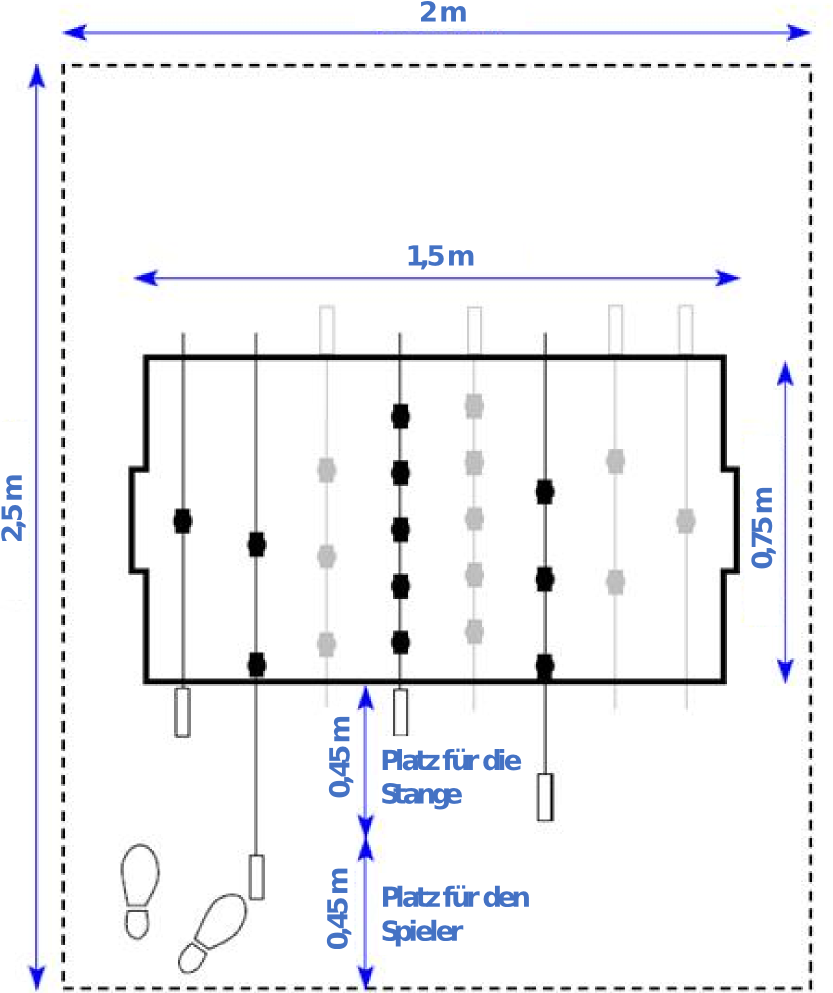
\includegraphics[width=\textwidth]{img/tisch_platzbedarf.png} 
\caption{Platzbedarf} 
\label{fig:tisch:platzbedarf} 
\vspace{0.5cm}
\end{subfigure} 
\begin{subfigure}[b]{0.7\textwidth} 
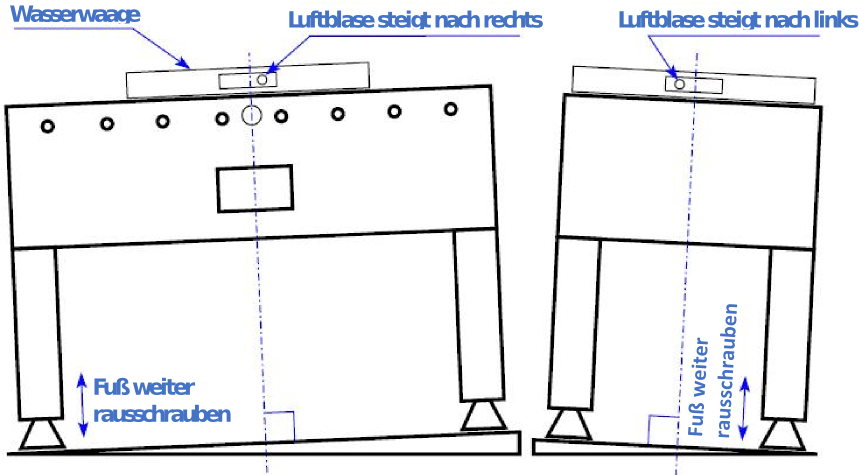
\includegraphics[width=\textwidth]{img/tisch_ausrichten.png} 
\caption{Ausrichten} 
\label{fig:tisch:ausrichten} 
\end{subfigure} 
\label{fig:tisch} 
\caption{Aufstellen eines Tischs [\cite{itsf_basics}]} 
\end{figure}
%\end{wrapfigure}

%%%%%%%%%%%%%%%%%%%%%%%%%%%%%%%%%%%%%%%%%%%%%%
\subsection{Pflege und Wartung}
\label{tisch:tisch:wartung}

Um einen gleichbleibenden Spielspaß zu haben, wird eine regelmäßige Tischpflege und Wartung empfohlen:
\begin{itemize}  
\item {\normalfont \bfseries Stangen:} Damit die Stangen leicht laufen, schmieren viele Spieler die Stangen mit Pronto-Spray (Möbelpolitur) oder Silikonöl, bevor Sie Tischfußball spielen. Dabei ist in jedem Fall darauf zu achten, die ganz herausgezogene oder ganz reingeschobenene Stange außerhalb des Tisches und nie über der Spielfläche zu beschmieren. Danach sollten die Stangen hin- und hergedreht werden, während man die Stange rein- und rauszieht, damit sich das Schmiermittel gut über die Stange verteilt  und die Stangen gut in den Lagern laufen.
Weitere Infos bei \href{http://ungeblogtkickern.blogspot.de/2014/11/wie-kann-ich-die-stangen-am-besten.html}{Ungeblogt}.
\item {\normalfont \bfseries Spielfeld:} Auf dem Spielfeld sammelt sich über die Zeit Schmutz wie bspw. Staub, abgelöste Gummistücke von den Puffern oder auch Ballspuren. Diese lassen sich am einfachsten und schonend mit etwas Glasreiniger und Haushaltspapier entfernen -- zumindest bei Soccer-Spielflächen wie bei Leonhart- oder Ullrich-Tischen. In jedem Fall sollte man auf Spülmittel und Scheuerschwämme verzichten. 
\item {\normalfont \bfseries Lager und Puffer:} Das Schmiermittel für die Stangen kann leider auch leicht Staub binden. Diese Masse setzt sich gerne in den Lagern über die Zeit ab. Mit einem zurechtgerollten normalen Schreib-Papier kann man die Ablagerungen durch Durchschieben der Rolle entfernen. Manchmal lohnt sich aber auch eine Grundreinigung und man baut die Figuren, Stangen und Lager aus, um die Lager ohne Stange gründlich zu reinigen. Dabei sollte man sich überlegen, ob man die Puffer ersetzt. Puffer lösen sich durch die Schmiermittel und die Belastung nach einiger Zeit auf.    
\item {\normalfont \bfseries Allgemeines:} Natürlich sollten alle Schrauben am Tisch fest sitzen. Es lohnt sich ab und zu zu überprüfen, ob alle Schrauben noch festsitzen.  
\end{itemize}  


%%%%%%%%%%%%%%%%%%%%%%%%%%%%%%%%%%%%%%%%%%%%%%
%%%%%%%%%%%%%%%%%%%%%%%%%%%%%%%%%%%%%%%%%%%%%%
\section{Bälle}
\label{tisch:baelle}

Es gibt verschiedene Typen von Bällen, obwohl der Durchmesser typischerweise 35 mm beträgt -- manchmal auch 34 mm \citep{www:kickerbau:baelle}.
Tischfußball-Bälle unterscheiden sich vor allem in ihrer Griffigkeit und ihrem Gewicht, zudem in ihrer Farbe und auch beim Material.
Insbesondere die Griffigkeit, und damit die Oberflächenbeschaffenheit des Balls, und das Gewicht sind entscheidend für die Spieleigenschaften.  

Vorgestellt werden hier drei Bälle, die auf den Soccertischen (Leonhart, Ullrich, Lettner) üblicherweise gespielt werden und alle aus weißem Plastik sind \citep{www:tfc-reutlingen}:
\begin{itemize}
\item Der Ullrich Ball:
Der Ullrich Ball ist durch seine eher weiche Oberfläche der griffigste Ball unter den Soccer-Bällen. 
Das ermöglicht eine Ballführung mit viel Kontrolle. Insbesondere beim Klemmen kann man damit den Ball an verschiedenen Punkten unter der Stange führen und spielen (siehe Kapitel \ref{technik:ballkontrolle:eine}).
% Grafik ? Foto 
Mit einem üblichen 35 mm Durchmesser wiegt der Ball 24 g.
Dadurch das der Ball relativ weich ist, bekommt er mit der Zeit Macken und Dellen, so dass ein langsamer Ball zum Teil nicht mehr ganz gerade rollt.
Er ist offizieller Ball in Deutschland und mit dem DTFB- und dem P4P-Schriftzug bedruckt.
\\
Preis: 2,00 Euro. 
\\
Spieler: Ab Anfänger bis Profi
\item Der Leonhart Ball: 
Mit einem Durchmesser von 35 mm und einem Gewicht von etwa 27 g ist im Vergleich zu vielen Bällen relativ schwer. 
Zusammen mit seiner harten und doch leicht griffigen Oberfläche hat er damit ruhiges und genaues Rollverhalten.
Er ist mit dem ITSF Schriftzug bedruckt, da er offizeller ITSF Ball für den Leonhart-Tisch ist.
\\
Preis: 2,50 Euro. 
\\
Spieler: Ab Fortgeschrittene bis Profi
\item Der Lettner Ball (Contus Avant):
Der dritte DTFB zertifizierte Ball ist für den Lettner Tisch entwickelt.
Er hat ein Gewicht von 27 g und einem Durchmesser von 34,9 mm.
Der Ball hat eine harte Oberfläche, ist jedoch leicht griffig. 
Er ist nicht so verbreitet wie der Leonhart- oder Ullrich-Ball. 
\\
Preis: 2,75 Euro.
\\
Spieler: Ab Amatuer bis Profi
\end{itemize}

Die Griffigkeit hängt nicht nur von der Art des Balls ab, sondern ist ein Zusammenspiel zwischen Figur, Ball und Spieloberfläche. 
Zum Beispiel spielt sich ein Leonhart-Ball auf einem Ullrich-Tisch eher weniger griffig.  
Und auch die offiziellen Tische -- die 5 ITSF- und 3 DTFB-Tische -- haben jeweils ihren eigenen zertifizierten Ball und dadurch unterschiedlichste Spieleigenschaften:
Der Bonzini-Ball ist orange und hart, aber auf dem Bonzini-Tisch sehr griffig. 
Im Gegensatz zum Tornado Ball, der aus roten Urethan ist, was ihn sehr hart und schwer macht -- und sehr ungriffig bzw. rutschig. 



%%%%%%%%%%%%%%%%%%%%%%%%%%%%%%%%%%%%%%%%%%%%%%
\section{Zubehör}
\label{tisch:zubehoer}

Das wichtigste Spielzubehör ist für eine gute Griffigkeit verantwortlich: \nameref{tisch:zubehoer:griffe}.
Auch auf angemessene \nameref{tisch:zubehoer:kleidung} legen Amateuer- und Profi-Spieler wert.
Zudem gibt es einige \nameref{tisch:zubehoer:training}, die für ein abwechslungsreiches und fokussiertes Trainieren sorgen können.

%%%%%%%%%%%%%%%%%%%%%%%%%%%%%%%%%%%%%%%%%%%%%%
\subsection{Griffbänder und Handschuhe}
\label{tisch:zubehoer:griffe}

Alle Spielaktionen beim Tischfußball geschehen durch die Hände der Spieler, die die Stangen über die Griffe bewegen.
Egal bei welcher \nameref{technik:haltung:griffe} und egal für welche Techniken ist eine gewisse Griffigkeit notwendig. 

Obwohl die festinstalliersierten Griffe bei den DTFB-Tischen (Leonhart, Ullrich, Lettner) aus schwarzem Gummi gurndsätzlich eine gute Griffigkeit bieten, kann sich die Griffigkeit bei längerem Spiel wegen Schwitzens verschlechtern.
Daher verwenden viele Spieler (Tennis-)Griffbänder, die sie vor dem Spielen um die Griffe wickeln. 
Griffbänder bieten zwei entscheidende Vorteile:
\begin{itemize}
\item Schweißabsorbtion und dadurch gleichbleibende Griffigkeit
\item besserer Griff beziehungsweise bessere Stangenkontrolle
\end{itemize}
Nach dem Spielen sollte man die Bänder wieder aufwickeln, damit die Oberfläche nicht einstaubt, und die Griffigkeit erhalten bleibt.
Manche Griffbänder kann man sogar mit in der Waschmaschine waschen, so dass diese nach längerer Benutzung wieder fast  wie neu sind. 
Griffbänder gibt es von vielen verschiedenen Herstellern und kosten etwa zwischen 0,50 und 2,50 Euro. 

\paragraph{Wie wickelt man ein Griffband auf?} Die Standardwicklung: 
\begin{itemize}
\item[a)] Man beginnt bei der tischnäheren Seite des Griffs und wickelt nach außen.
Man sollte darauf achten, dass der Bandanfang durch die ersten Wicklungen fixiert wird. 
\item[b)] Durch Drehen der Stange wickelt man das Band gleichmässig auf den Griff, wobei das Band stets etwa zur Hälfte die darunter leigende Schicht überdecken sollte.
\item[c)] Ist das Band ganz aufgewickelt, benutzt man ein Abschlussgummi, um die letzte Wicklung zu fixieren.
\end{itemize}
Video-Link: \url{https://www.youtube.com/watch?v=KgOqDdcp4n4}


Ein ebenfalls beliebtes Zubehör sind (Golf-)Handschuhe. 
Damit kann man insbesondere in Kombination mit Griffschläuchen oder -gummis, die man über den Griff zieht, eine erhöhte Griffigkeit erlangen.
Dieses Material ist bei Spielern, die mit der Abroller-Technik schießen, besonders beliebt, da man mit wenig Druck auf die Stange, dennoch eine hohe Seitwärts-Bewegung erreichen kann (siehe Kapitel \ref{technik:torschuesse}).  

Spieler, die Jet schießen, benutzen Material um ihre Handgelenke bzw. den Unterarm. 
Manche benutzen dafür ein verkürztes Griffband bzw. eigens dafür hergestellte Jet-Armbänder.
Dadurch soll ebenfalls eine schnelle Seitwärts-Bewegung erreicht werden, bei wenig Kraftaufwand (siehe Kapitel \ref{technik:torschuesse}).

\paragraph{Hintergrund:} Da sich die Griffe der 5 offiziellen ITSF-Tische in Dicke und Form, Material und Griffigkeit unterscheiden, wurde vor einigen Jahren ein Griffwechselsystem bei internationalen Turnieren eingeführt.
Das ermöglicht den Spielern ihren Lieblingsgriff an allen Tischen zu spielen. 

\paragraph{Weitere Infos} bei \href{http://ungeblogtkickern.blogspot.de/2015/05/griffe-praparieren.html}{Ungeblogt}.

%%%%%%%%%%%%%%%%%%%%%%%%%%%%%%%%%%%%%%%%%%%%%%
\subsection{Kleidung}
\label{tisch:zubehoer:kleidung}

Nach dem ITSF-Regelwerk gibt es beim Tischfußball einen Dresscode, der Sportkleidung vorschreibt. 
Bei internationalen und nationalen Wettkämpfen tragen die Spieler Trikots mit ihrem Vereinslogo und ihrem Namen darauf. 
Neben der Teamzugehörigkeit bieten Sporttrikots eine gewisse Atmungsaktivität, die bei einem schweisstreibendem Spiel von Vorteil sind. 
Manche Spieler haben sogar ein Handtuch in Tischnähe, um Ihren Schweiss in Auszeiten abzuwischen.

Während eines Turniertages ziehen sich viele Spieler, zwischen den Spielen eine Trainingsjacke an, um nicht auszukühölen.
Bei der Hosenwahl -- ob kurz oder lang -- ist es den Spielern überlasssen, wie man sich am wohlsten fühlt. 
Bei der Schuhwahl sollte man darauf achten, dass man beim Tischfußball überwiegends steht. 
Daher wird ein wohlfühlendes Schuhbett empfohlen, wie etwa ein gut gedämpfter Laufschuh.  

%%%%%%%%%%%%%%%%%%%%%%%%%%%%%%%%%%%%%%%%%%%%%%
\subsection{Trainingsmaterialien}
\label{tisch:zubehoer:training}

%%%%%%%%%%%%%%%%%%%%%%%%%%%%%%%%%%%%%%%%%%%%%%
\subsubsection{Stangenklemmen oder Rod-Locks}
\label{tisch:zubehoer:training:rodlock}

\begin{figure}
%\begin{wrapfigure}{r}{0.4\textwidth} 
\centering 
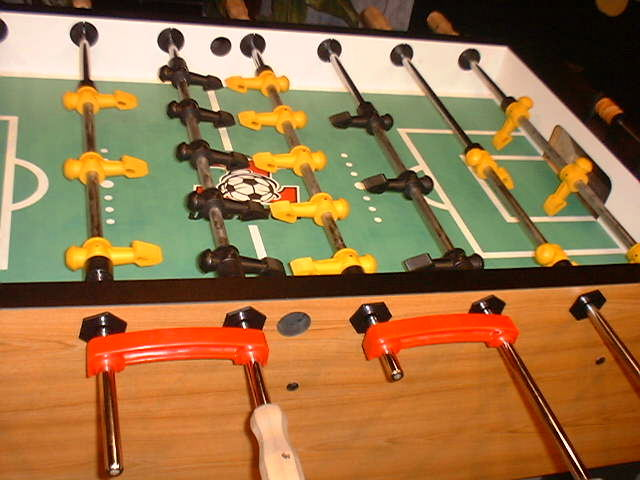
\includegraphics[width=0.38\textwidth]{img/rodlock_goalie.jpg} 
\caption{Um ein Goalie-Einzel zu spielen, verbindet hier eine rote Stangenklemme die gelbe 3er- mit der schwarzen 5er-Reihe und eine zweite Klemme die gelbe 5er- mit der schwarzen 3er-Reihe. [\cite{www:rod-lock}]} 
\label{fig:rod-lock} 
\end{figure}
%\end{wrapfigure}

Stangenklemmen, oder im Englischen Rod-Locks, sind wohl das gängigsten Trainingszubehör. 
Eine Klemme kann an zwei Stellen an eine Stange geklemmt werden, so dass sich zwei Stangen miteinander fixiert werden können. 
Damit ergeben sich folgende Trainingsvarianten \citep{www:rod-lock}:
\begin{itemize}
\item \nameref{spielformen:sonderregeln:goalie}: Mit zwei Stangenklemmen kann man die Mittelfeld- und Sturmreihen hochklappen, so dass die Spielfiguren waagrecht bleiben (siehe Abb.~\ref{fig:rod-lock}). 
Somit kann man Torwart gegen Torwart spielen. 
\\
Zielgruppe: ab Anfänger
\\
Trainingseffekt: Torwartdasein
\item Schusstraining: Mit einer Klemme kann man die Torwart- und 2er-Stange festklemmen. 
Durch Variation der Distanz zwischen Torwart- und Abwehrfigur sowie deren Stellungswinkel kann man verschiedene statische Deckungen stellen.
Dadurch kann trainieren auf verschiedene Lücken Tore zu schießen.  
\\
Zielgruppe: ab Fortgeschrittene
\\
Trainingseffekt: Hand-Auge-Koordination, Präzession beim Schiessen
\item Mittelfeldtraining: Eine Stangenklemme and die gegnerische Mittelreihe einseitig geklemmt, so dass die Figuren nach vorne gestellt sind, wenn die Klemme nach unten hängt, ist für ein Mittelfeldtraining effektiv:
Beim Passtraining von der 5er- auf die 3er-Stange versucht man durch die gegnerische 5er-Reihe zu spielen. 
Trifft man die gegnerische Figur, wird der Ball durch das Auslenken der Stangenklemme automatisch zurückgespielt, so dass man zum Einen lernt die Abpraller zu kontrollieren und zum Anderen gleich den nächsten Passversuch spielen kann, ohne den Ball mit der Hand zurechtzulegen.
\\
Zielgruppe: ab Amateurspieler
\\
Trainingseffekt: Mittefeldspiel, Präzession beim Passen
\end{itemize}
Eine Stangenklemme kostet 10 bis 20 Euro.

Für das \nameref{spielformen:sonderregeln:goalie} kann man zwei Stangen auch mit einem einfachen Haushaltsgummi hochstellen.
Dafür legt man den Gummi um den Kopf einer Figur (z.B. die mittlere Figur der 3er-Reihe), dreht dann das andere Ende des Gummis um eine halbe Umdrehung und legt dieses um des Kopf der Figur an der zweiten Stange (z.B. die mittlere Figur der 5er-Reihe). 

%%%%%%%%%%%%%%%%%%%%%%%%%%%%%%%%%%%%%%%%%%%%%%
\subsubsection{Weiteres Zubehör}
\label{tisch:zubehoer:training:weiteres}

\begin{itemize}
%%%%%%%%%%%
\item {\normalfont \bfseries Backbouncer:}
Der Backbouncer ist aus Holz gebaute U-Form, die die Länge einer Tischbreite hat \citep{www:kickertrainer}.
An einer Seite ist ein elastischer Zellkautschuk angebracht.
Die U-Form lässt sich um jede Stange und deren Figuren stellen. 
Damit prallt der Ball zurück, wenn man diesen gegen den Kautschuk schiesst: 
Man kann alleine üben, abgeprallte Bälle zu stoppen und zu kontrollieren, in dem man verschieden stark und mit unterschiedlichen Winkeln gegen den Kautschuk spiel. 
Den Backbouncer gibt es auch mit einem zackig geschnittenen Kautschuk, so dass der Ball unvorhergesehen abprallt.  
\\
Zielgruppe: ab Anfänger 
\\
Trainingseffekt: Hand-Auge-Koordination, Reaktion, Ballgefühl
%%%%%%%%%%%
\item {\normalfont \bfseries FoosTrain:}
Mit Federn verbindet man die 2er- und die 3er-Stange \citep{www:foostrain}.
Sobald man eine Seitwärts-Bewegung macht, folgt die Abwehrstange der Bewegung, so dass man schnell genug zum Schuss kommen muss, um nicht von der heranfahrenden Abwehrfigur gehalten zu werden.
Durch größere Federstärken erhöht man den Schwierigkeitsgrad, da die Abwehrstange schneller der Bewegung folgt.
\\
Zielgruppe: ab Fortgeschrittene
\\
Trainingseffekt: Schusstechnik und Bewegungsablauf 
%%%%%%%%%%%
\item {\normalfont \bfseries Table Soccer Coach oder Visual-Kickertrainer:}
Der Table Soccer Coach ist eine Smart-Phone App \citep{www:tablesoccercoach}:
Man legt das Gerät über das Tor und startet das Programm. 
Nach einer zufälligen Zeit erscheint dann ein Signal und man muss schießen.
Neben dem akkustischen Signal gibt es noch ein visuelles Signal auf dem Display, das anzeigt, welche Lücke man schießen soll.
Ähnlich funktioniert der Visual-Kickertrainer, der durch eine LED-Leiste realisiert ist \citep{www:visualkickertrainer}.
\\
Zielgruppe: ab Amateurspieler 
\\
Trainingseffekt: Abrufbarkeit der Schüsse, Entscheidungsgeschwindigkeit
\\
Weitere Infos bei \href{http://ungeblogtkickern.blogspot.de/2015/01/table-soccer-coach.html}{Ungeblogt}.

%%%%%%%%%%%
\item {\normalfont \bfseries Kickertrainer:}
Der Kickertrainer ist im Prinzip ein verkürzter Tisch: Das Spielfeld ist 3 Stangen lang \citep{www:kickertrainer}. 
Damit kann man ihn schnell auf- und abbauen und zu Hause unterbringen, falls man nicht den Platz für einen Kickertisch hat.
Zudem kann man sich mittels Holzplättchen verschiedene Lücken stellen, durch die man Passen oder Schiessen muss. 
\\
Zielgruppe: ab Anfänger 
\\
Trainingseffekt: Präzession beim Passen und Schiessen
%%%%%%%%%%%
\item {\normalfont \bfseries Kicker Maschine:} 
Die Kicker Maschine ist eine junge Entwicklung, die es noch nicht zu kaufen gibt, aber eine interessante Trainingsmöglichkeit bietet \citep{www:kickermaschine}. 
Durch ein Motor-betriebenes Hebelsystem werden die gegnerischen Stangen automatisch hin- und herbewegt. 
Dadurch kann man das Passen und Schiessen üben, während sich die gegnerischen Stangen rythmisch bewegen.
\\
Zielgruppe: ab Amateuerspieler 
\\
Trainingseffekt: Deckungsanalyse und Timing

\end{itemize}
